\chapter{Implementación}
En el modelo ``cascada'' la fase de implementación es la más importante, debido a que en esta se desarrolla el producto final a partir del diseño de la fase anterior. El diseño previo permite al programador implementar con éxito los diferentes módulos del sistema de video-vigilancia planteado. El desarrollo de todo el sistema esta programado con el lenguaje de programación Python ne su totalidad.

\section{Módulo de Cámaras}
A partir del diseño inicial se implementa la interfaz de usuario por medio de la libreria ``tkinter'' propia del lenguaje. En la figura \ref{fig:camera_screen}, se visualiza la implementación final en base al diseño de la fase anterior de la metodología.\\

\begin{figure}[H]
    \begin{center}
        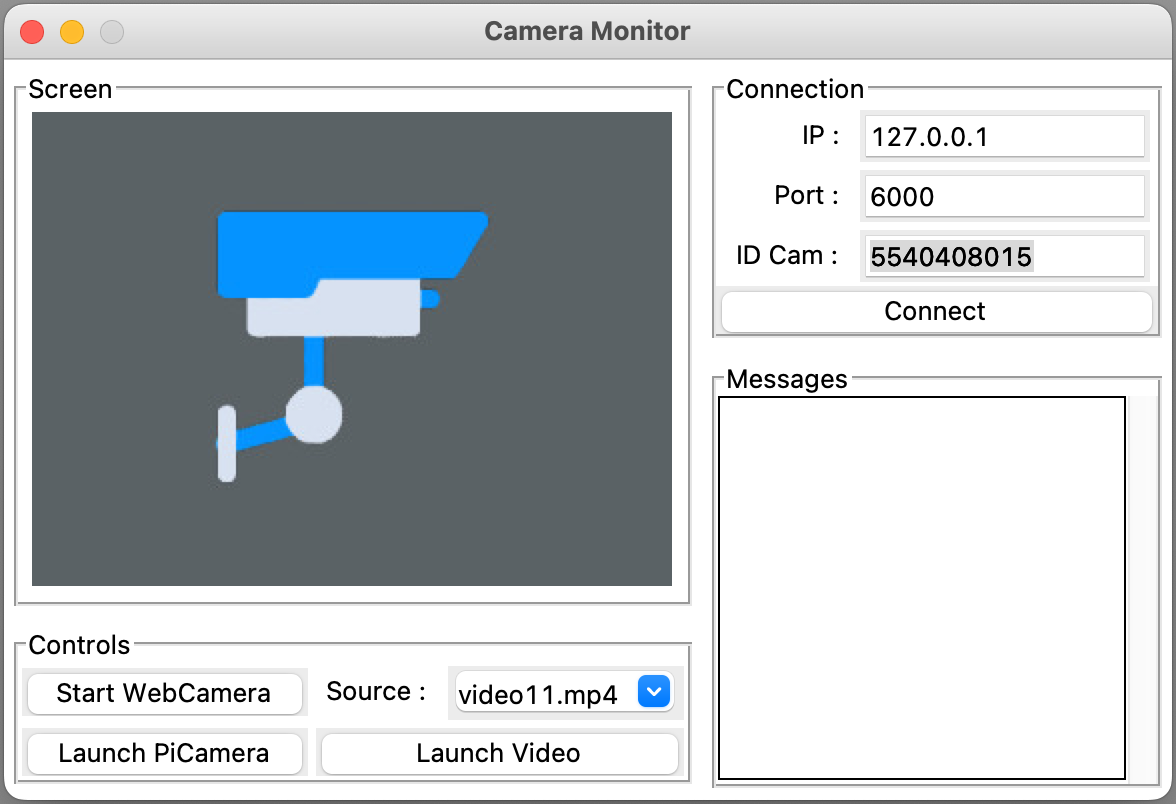
\includegraphics[width=12cm]{img/capitulo_5/camera_interface.png}
        \caption{Interfaz gráfica del módulo de cámaras.}
        Fuente : Elaboración Propia.
        \label{fig:camera_screen}
    \end{center}
\end{figure}

La conexión entre el módulo de cámaras y el servidor se realiza por medio de otro paquete propio del lenguaje denominado ``sockets'', que es utilizado para el envio de mensajes por medio de la red. En la figura \ref{fig:socket_client} se visualiza el código necesario para el envio de un fotograma al servidor.

% \lstset{style=mystyle}
% \begin{lstlisting}[language=Python]
%     def send_frame(self, frame, quality):
%         encode_param = [int(cv2.IMWRITE_JPEG_QUALITY), quality]
%         result, image = cv2.imencode('.jpg', frame, encode_param)
%         data = pickle.dumps(image, 0)
%         if self.is_connected():
%             try:
%                 self.__socket_connected__.\
%                     sendall(struct.pack(">L", len(data)) + data)
%             except socket.error:
%                 message = self.receive_message_connection_rejected()
%                 self.__controller__.disconnect_to_server()
% \end{lstlisting}

\begin{figure}[H]
    \begin{center}
        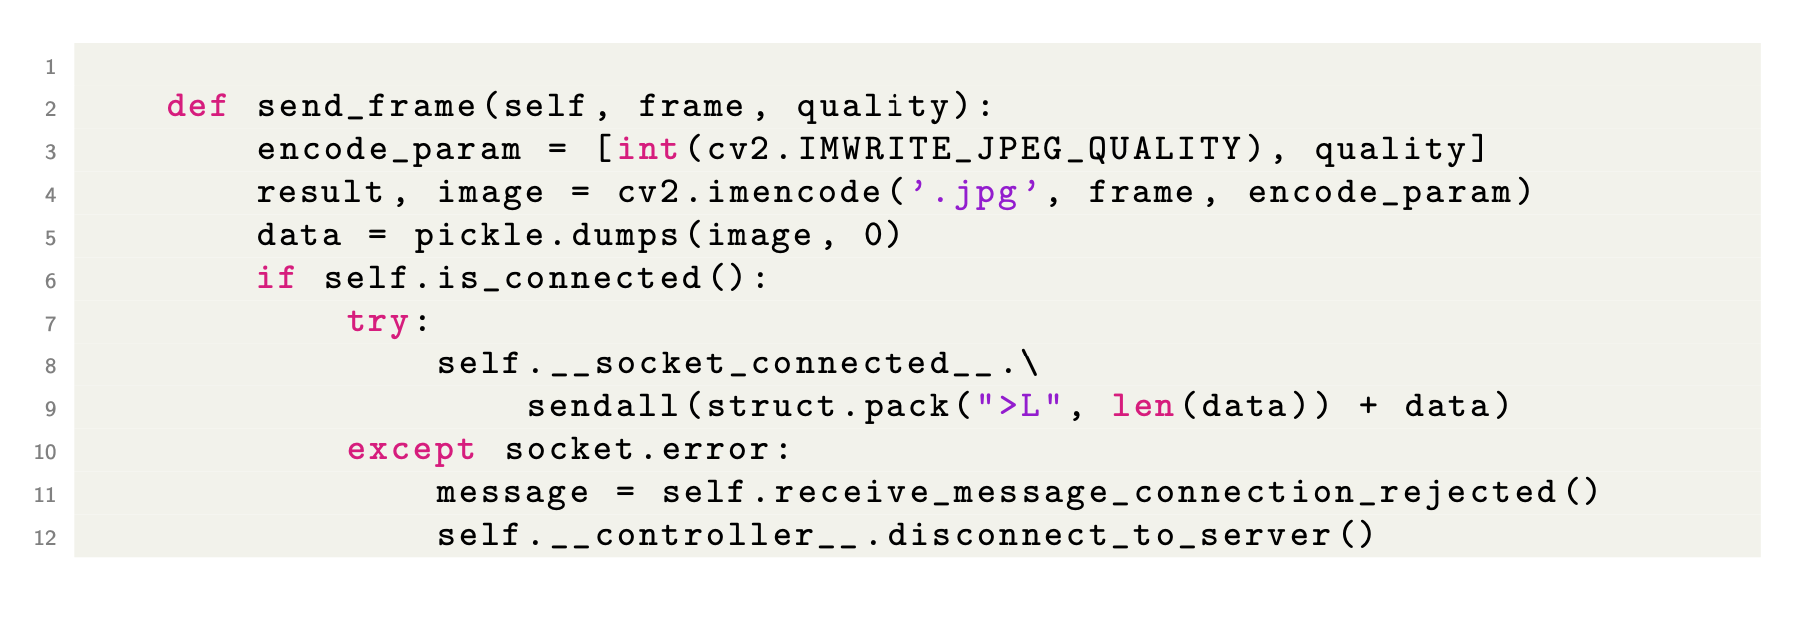
\includegraphics[width=15cm]{img/capitulo_5/code1.png}
        \caption{Código de envío de un fotograma por medio de sockets.}
        Fuente : Elaboración Propia.
        \label{fig:socket_client}
    \end{center}
\end{figure}

Para que el fotograma sea enviado por la red este debe ser serializado y convertido en un paquete de datos binario y esto es logrado con el uso de los paquetes pickle y struct en las líneas 5 y 9 respectivamente.\\

Cuando el módulo de cámaras y el servidor se conectan, si inicia el proceso de envío de fotogramas hacia el servidor, y este es visualizado y numerado por cada fotograma enviado, en el campo de mensajes del sistema propio de la interfaz gráfica del módulo de cámaras. Este comportamiento se visualiza en la figura \ref{fig:working_camera}.

\begin{figure}[H]
    \begin{center}
        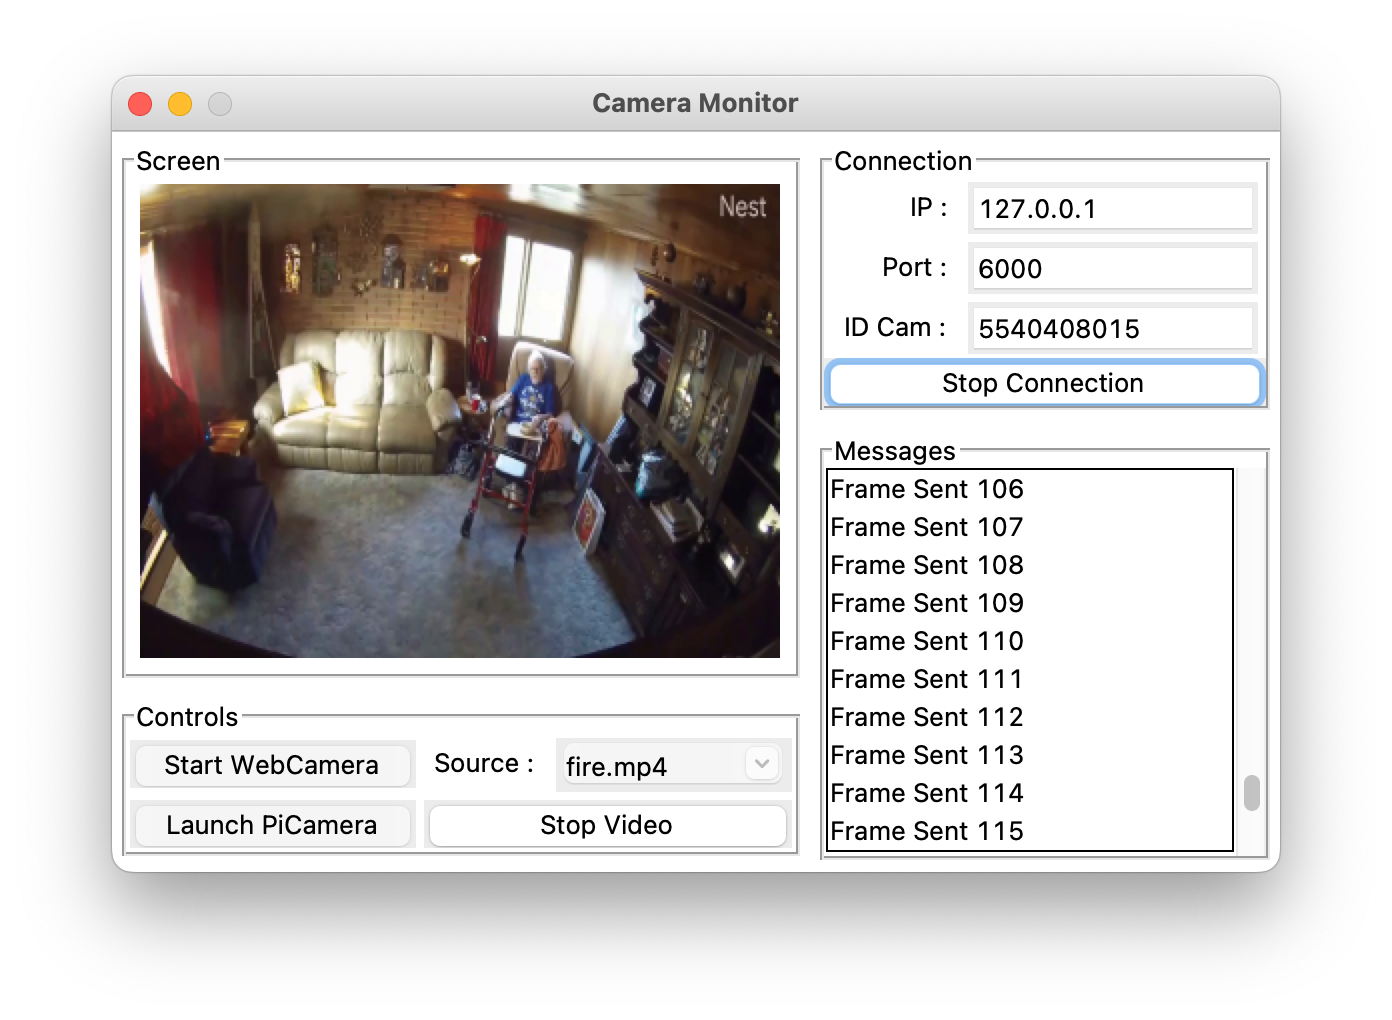
\includegraphics[width=13cm]{img/capitulo_5/camera_working.png}
        \caption{Interfaz gráfica del módulo de cámaras en envio de fotogramas.}
        Fuente : Elaboración Propia.
        \label{fig:working_camera}
    \end{center}
\end{figure}


\section{Módulo de servidor}
Es el módulo central que gestiona distintos procesos como ser: 
\begin{itemize}
    \item Gestión de conexiones del módulo de cámaras.
    \item Recepción de fotogramas recibidos.
    \item Análisis de fotogramas según algoritmos de visón artificial.
    \item Notificación por correo electrónico.
\end{itemize}
\subsection{Interfaz de consola}
Durante la ejecución del servidor es necesario visualizar el estado del mismo. La opcion inmediata y práctica es manejar mensajes del servidor por medio de la consola del sistema operativo. En la figura \ref{fig:servertcp_console} se visualiza un ejemplo del estado inicial del servidor.\\

\begin{figure}[H]
    \begin{center}
        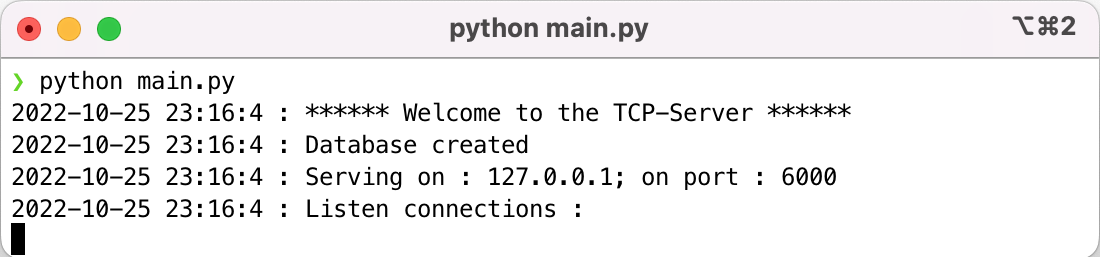
\includegraphics[width=10cm]{img/capitulo_5/tcp_server.png}
        \caption{Ejecución del servidor TCP.}
        Fuente : Elaboración propia
        \label{fig:servertcp_console}
    \end{center}
\end{figure}
Además de registrar cada mensaje en pantalla se agrega la fecha y hora de su lanzamiento como se aprecia en la figura anterior.
\subsection{Configuración y conexiones}
Para la ejecución inicial del servidor es necesario ingresar las configuraciones relevantes para un funcionamiento consistente. Para tal objetivo se prevee de un archivo inicial de configuración en el cual se registran todos los valores en los que se basará el servidor. En la figura \ref{fig:config_file} se visualiza el archivo de configuración del servidor.\\

\begin{figure}[H]
    \begin{center}
        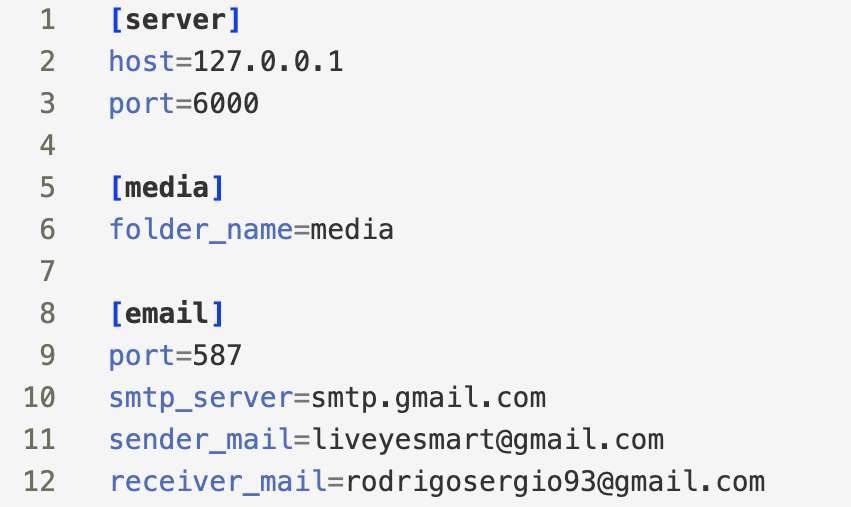
\includegraphics[width=6cm]{img/capitulo_5/config.ini.png}
    \end{center}
    \begin{center}
        \caption{Archivo de configuración del servidor.}
        Fuente : Elaboración propia
        \label{fig:config_file}
    \end{center}
\end{figure}

Este archivo permite definir información sobre el nombre del servidor, puerto de escucha y valores relevantes para la notificación por correo electrónico.\\

Las conexiones son gestionadas tambien por el servidor manteniendo informado al usuario sobre las nuevas conexiones por medio de la interfaz de consola como tambien por notificación que sera descrito más adelante. En la figura \ref{fig:server_messages} se visualiza los diferentes mensajes referentes a las conexiones por parte de la interfaz de consola.\\

\begin{figure}[H]
    \begin{center}
        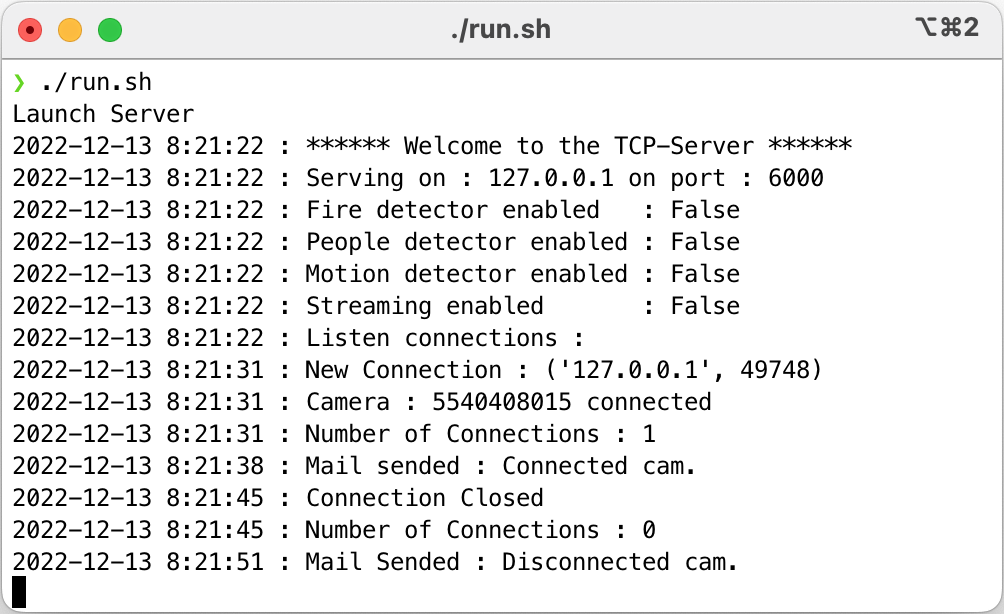
\includegraphics[width=12cm]{img/capitulo_5/server_messages.png}
    \end{center}
    \begin{center}
        \caption{Mensages de consola del servidor.}
        Fuente : Elaboración propia
        \label{fig:server_messages}
    \end{center}
\end{figure}

\subsection{Análisis de fotogramas}
La característica central de este sistema de video-vigilancia es la detección de diferentes sucesos con el uso de algoritmos de visión por computadora e intelgencia artificial. A continuación se describen los algoritmos encargados para cada detección.\\
\subsubsection{Detector de Fuego}
Es el encargado de identificar la presencia de fuego en los fotogramas que recibe el servidor. La detección que realiza hace uso de detectores en ``cascada'', que es un enfoque basado en Aprendizaje Automático en la que la función cascada se entrena a partir de muchas imágenes positivas y negativas, para luego utilizar este entrenamiento para realizar la detección en otro conjunto de imágenes.\\

La libreria de visión por compuradora ``OpenCV'' permite cargar los archivos .xml, que representan el entrenamiento, a su método HaarCascade, encargado de procesar la imágen. En la figura \ref{fig:fire_detector} se visualiza el código central de la detección de fuego, donde se aprecia el cargado del archivo de entrenamiento para el clasificador.\\


% \lstset{style=mystyle}
% \begin{lstlisting}[language=Python]
% def detector(connection):
%     fire_cascade = cv2.CascadeClassifier(
%         'detectors/fire_detection.xml'
%     )
%     while connection.running:
%         frame, label = connection.get_frame(objetive='fire_detector')
%         if frame is not None:
%             fire = fire_cascade.detectMultiScale(
%                 image=frame,
%                 scaleFactor=1.1,
%                 minNeighbors=3,
%                 flags=0
%             )        
%             if len(fire) > 0:
%                 connection.fire_detections.append((frame, label))
% \end{lstlisting}

\begin{figure}[H]
    \begin{center}
        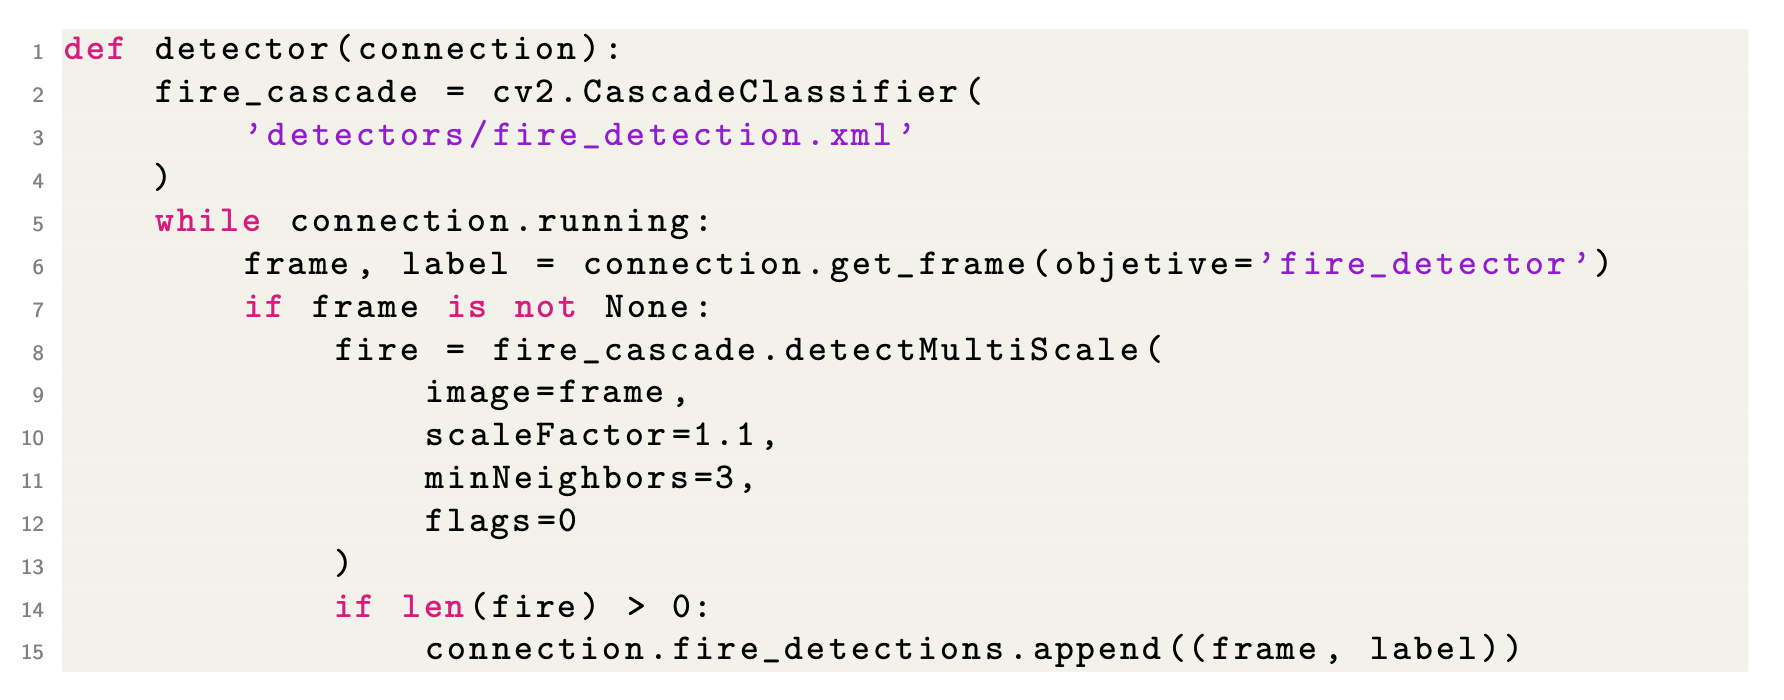
\includegraphics[width=18cm]{img/capitulo_5/fire_detector.png}
    \end{center}
    \begin{center}
        \caption{Código de detección de fuego.}
        Fuente : Elaboración propia
        \label{fig:fire_detector}
    \end{center}
\end{figure}

El clasificador realiza una detección multi-escala en base a los valores que se asignan al método en las líneas 10, 11 y 12.\\

\subsubsection{Detector de silueta humana}
Es el encargado de la detección de intrusos por la silueta humana, en base a los fotogramas recibidos por el servidor. Este detector hace uso del algoritmo HOG (Histograma de gradiente orientado) implementado por la libreria ``OpenCV''. Este método es entrenado para detectar gente que camina, que en la mayoria de los casos están de pie, asi que no se espera que funcione correctamente en otros casos.
La idea básica del método es la siguiente:\\

\begin{itemize}
    \item La imágen se escanea con una ventana de detección de tamaño variable.
    \item Para cada posición y tamaño de la ventana de detección, esta se subdivide en celdas. Estas celdas son relativamente pequeñas: típicamente contienen solo una pequeña parte de la persona a detectar, tal vez el costado de un brazo o la parte superior de la cabeza.
    \item En cada celda, se calcula un gradiente para cada píxel y los gradientes se utilizan para llenar un histograma: el valor es el ángulo del gradiente y el peso es la magnitud del gradiente.
    \item Los histogramas de todas las celdas se juntan y se envían a un discriminador de aprendizaje automático para decidir si las celdas de la ventana de detección actual corresponden a una persona o no.
\end{itemize}

En la figura \ref{fig:human_detector} se visualiza el código del detector de silueta huamana.\\

\begin{figure}[H]
    \begin{center}
        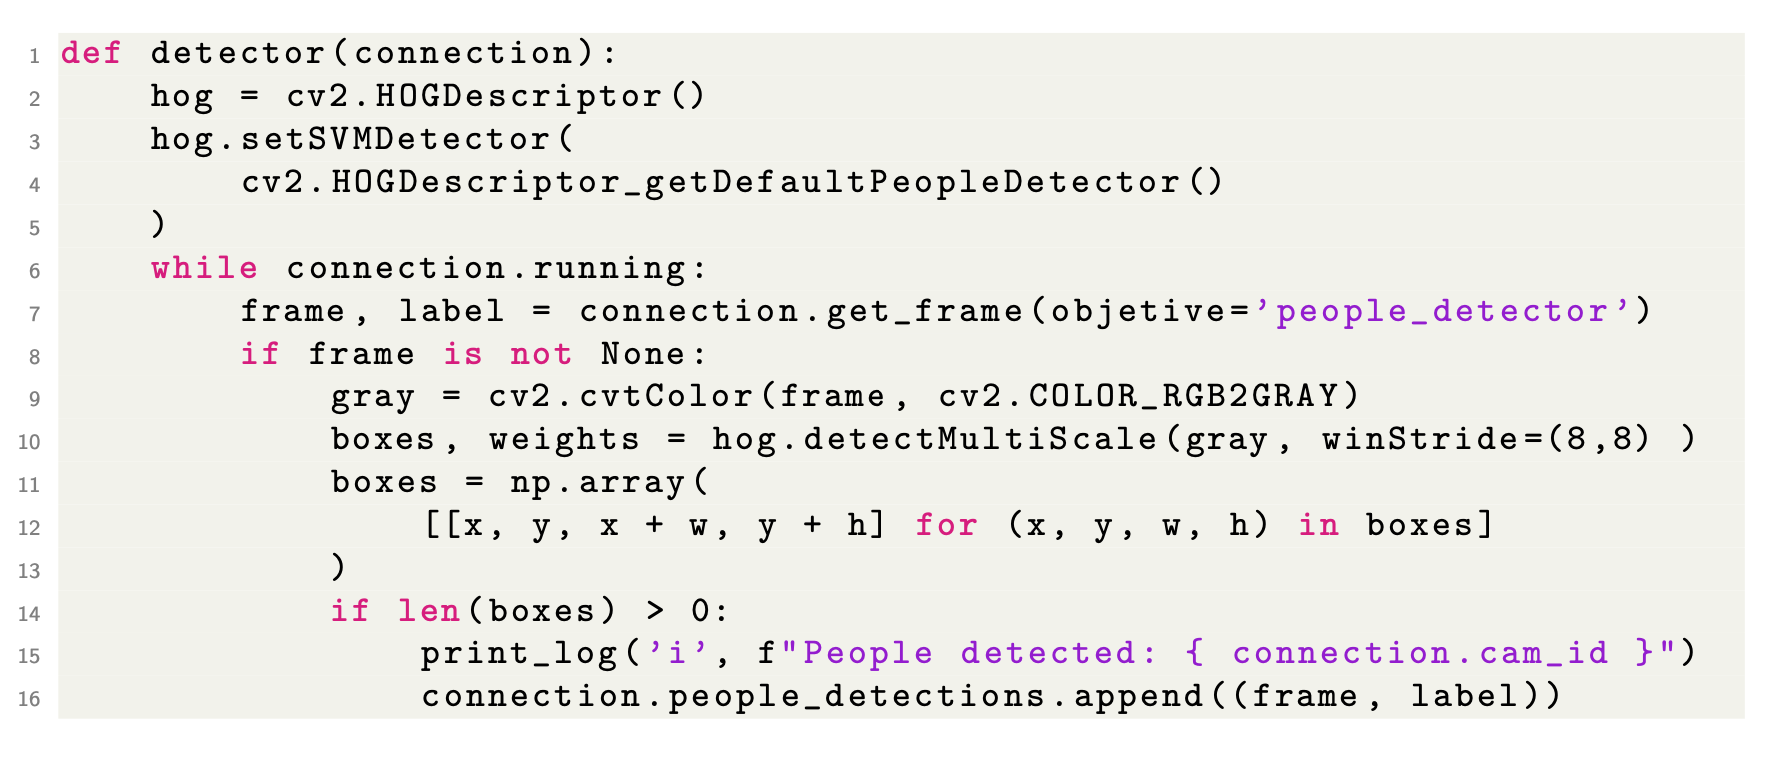
\includegraphics[width=16cm]{img/capitulo_5/human_detector.png}
    \end{center}
    \begin{center}
        \caption{Código de detección de silueta humana.}
        Fuente : Elaboración propia
        \label{fig:human_detector}
    \end{center}
\end{figure}

% \lstset{style=mystyle}
% \begin{lstlisting}[language=Python]
% def detector(connection):
%     hog = cv2.HOGDescriptor()
%     hog.setSVMDetector(
%         cv2.HOGDescriptor_getDefaultPeopleDetector()
%     )
%     while connection.running:
%         frame, label = connection.get_frame(objetive='people_detector')
%         if frame is not None:
%             gray = cv2.cvtColor(frame, cv2.COLOR_RGB2GRAY)
%             boxes, weights = hog.detectMultiScale(gray, winStride=(8,8) )
%             boxes = np.array(
%                 [[x, y, x + w, y + h] for (x, y, w, h) in boxes]
%             )
%             if len(boxes) > 0:
%                 print_log('i', f"People detected: { connection.cam_id }")
%                 connection.people_detections.append((frame, label))
% \end{lstlisting}

\subsubsection{Detector de movimiento}
Encargado de la detección de movimiento en base a los fotogramas recibidos por el servidor. El detector hace uso de métodos implementados en la libreria ``OpenCV''. En la figura \ref{fig:motion_detector} se detalla el código implementado que hace uso de métodos propios de la libreria.\\

% \lstset{style=mystyle}
% \begin{lstlisting}[language=Python]
% def detector(connection):
%     static_back = None
%     while connection.running:
%         frame, label = connection.get_frame(objetive='motion_detector')
%         if frame is not None:
%             gray = cv2.cvtColor(frame, cv2.COLOR_BGR2GRAY)
%             gray = cv2.GaussianBlur(gray, (21, 21), 0)
%             if static_back is None:
%                 static_back = gray
%                 continue
%             diff_frame = cv2.absdiff(static_back, gray)
%             thresh_frame = cv2.threshold(
%                 diff_frame, 30, 255, cv2.THRESH_BINARY)[1]
%             thresh_frame = cv2.dilate(
%                 thresh_frame,
%                 None, 
%                 iterations=3)
%             cnts, _ = cv2.findContours(
%                 thresh_frame.copy(), 
%                 cv2.RETR_EXTERNAL, 
%                 cv2.CHAIN_APPROX_SIMPLE)
%             if len(cnts) > 0:
%                 connection.motion_detections.append((frame, label))
% \end{lstlisting}
\begin{figure}[H]
    \begin{center}
        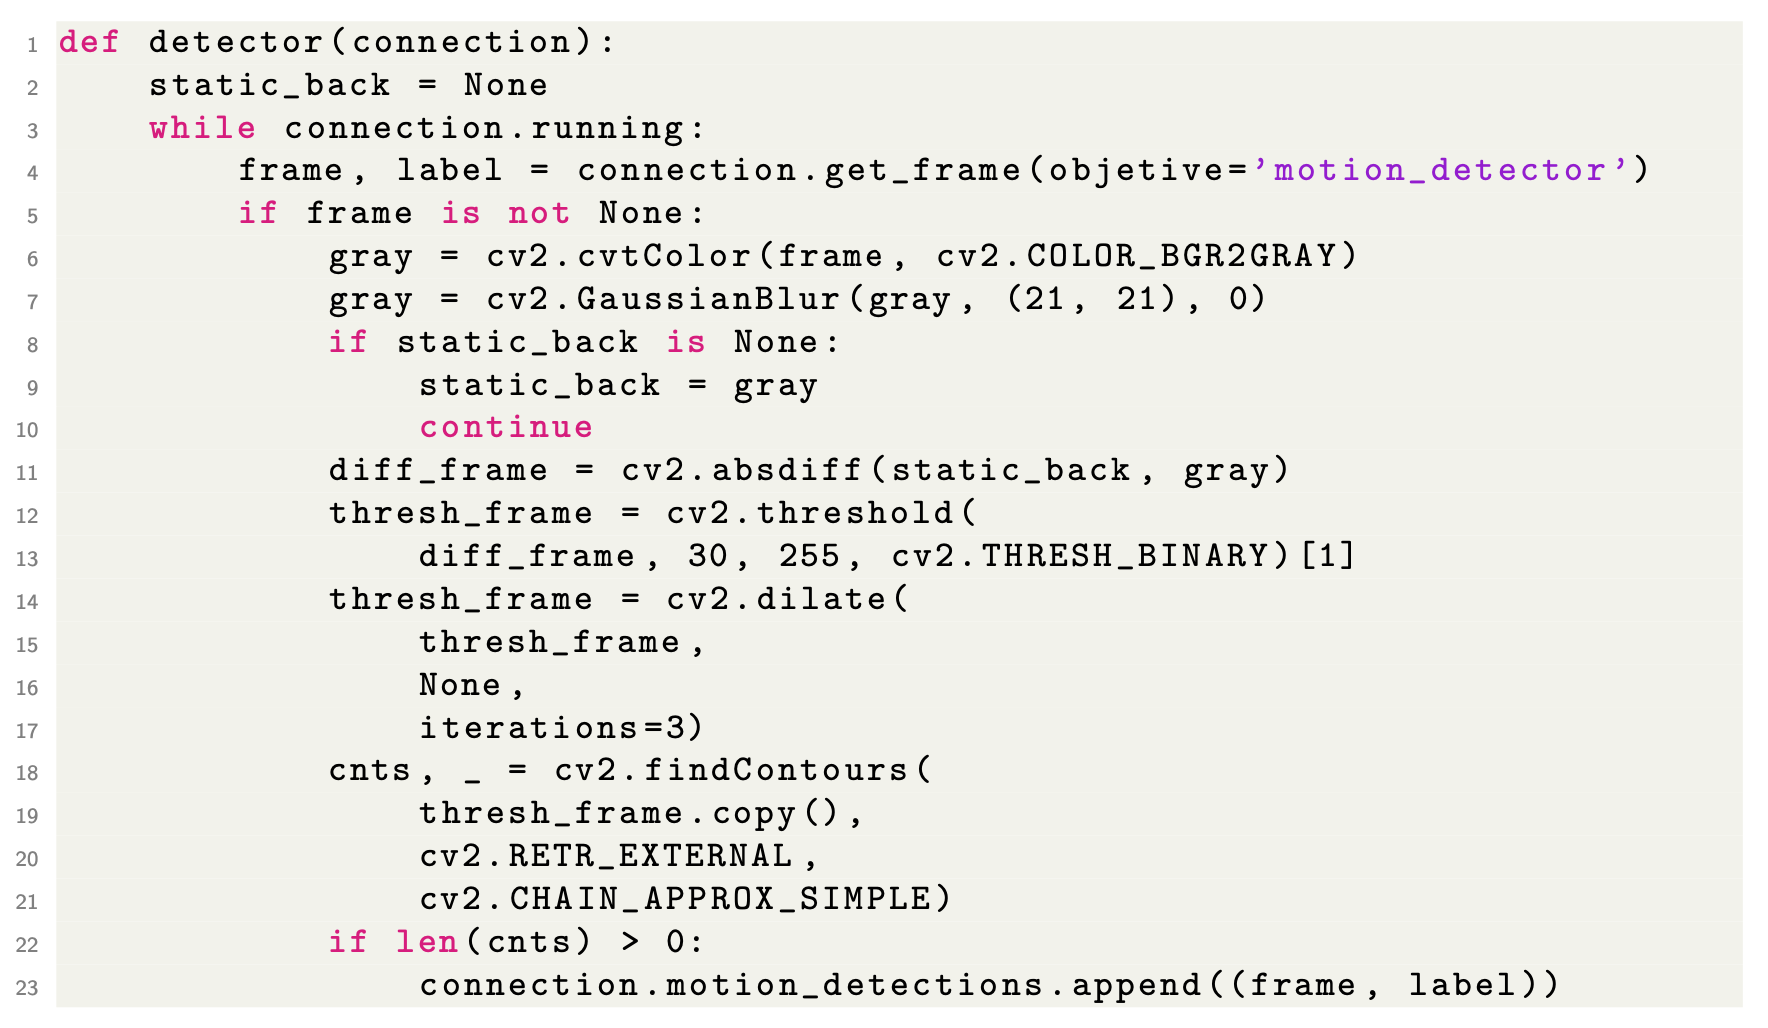
\includegraphics[width=16cm]{img/capitulo_5/motion_detector.png}
    \end{center}
    \begin{center}
        \caption{Código de detección de movimiento.}
        Fuente : Elaboración propia
        \label{fig:motion_detector}
    \end{center}
\end{figure}

El método implementado convierte el fotograma a otro en escala de grises, aislando el color dureante la detección. Define el primer fotograma como referencial para comparar con los siguientes fotogramas y determinar posibles diferencias que sugieren un movimiento.\\ 
\subsection{Transmisión de video en vivo}
Se implementa la clase que maneja la libreria ``VidGear'' encargada de realizar la decodificación y codificación de video generando el archivo que indexa las porciones de archivos multimedia, generados por el proceso para su transmisión. En la figura \ref{fig:vidgear} se detalla los valores de configuración necesaria para la correcta ejecución de la libreria, especificando la resolución y el framerate del video a generar.\\

% \lstset{style=mystyle}
% \begin{lstlisting}[language=Python]
% stream_params = {
%     "-input_framerate": frame_rate,
%     "-livestream": True,
%     "-streams": [{
%                 "-resolution": "640x360",
%                 "-framerate": "30.0"}]
% }
% self.streamer = StreamGear(output = output_path, format = output_format, **stream_params
% )
% \end{lstlisting}
\begin{figure}[H]
    \begin{center}
        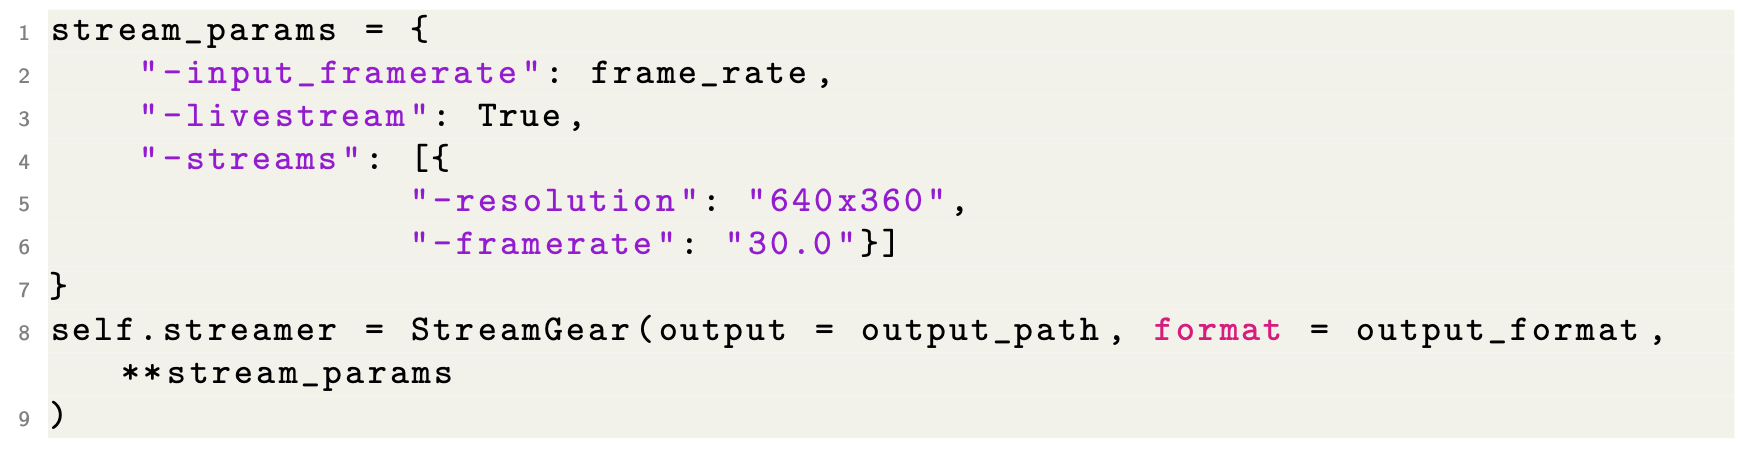
\includegraphics[width=16cm]{img/capitulo_5/vidgear.png}
    \end{center}
    \begin{center}
        \caption{Código de de configuración de la libreria VidGear.}
        Fuente : Elaboración propia
        \label{fig:vidgear}
    \end{center}
\end{figure}
